%!TEX program = xelatex
\documentclass[letterpaper,12pt]{exam}
\usepackage{../videoNotes}
\usepackage{float}
\usepackage{xcolor}
\usepackage[dvipsnames]{xcolor}
\usepackage{soul}
%\usepackage{draftwatermark}
\usepackage{multicol}
\usepackage[margin=5mm]{geometry}
\usepackage{fontspec}
\usepackage{tabulary}
\setmainfont{Noto Sans}
\setmonofont{Noto Sans Mono}
%\SetWatermarkText{DRAFT}
%\SetWatermarkScale{1.5}
%\SetWatermarkColor{red!20}
\newcommand{\unit}{Exam 2 Cheatsheet \textcolor{red}{DRAFT}}
\pagestyle{headandfoot}
\begin{document}
\section*{\unit}
\section*{Syscall}
\begin{tabular}{| c | c | c | c| c |}
 \hline
    rax & System Call & rdi & rsi & rdx \\
    \hline
    $0$ & read & file descriptor & buffer & number of bytes \\
    \hline
    $1$ & write & file descriptor & buffer & number of bytes \\
    \hline
    $60$ & exit & exit code & --- & --- \\
    \hline
\end{tabular}
\par
\section*{Calling C library functions}

\begin{itemize}
    \item Parameters are stored in registers in the following order: rdi, rsi, rdx, rcx, r8, r9. (If there are more parameters, they are pushed onto the stack)
    \item Most C functions return an integer or a pointer (which is just an integer).  The return value is placed in the rax register
    \item The called functions may use or destroy the content of the following registers: rax, rcx, rdx, rsi, rdi, r8, r9, r10, r11 
    \item Other registers may be used, but the called function is responsible for saving them.
\vspace{15 mm}

\end{itemize}
\par

\begin{center}
\begin{tabulary}{\textwidth}{C C C C C C C}
\multicolumn{7}{c}{{\huge General Purpose Registers}}\\
64-bit & 32-bit & 16-bit & 8-bit low & 8-bit high & Calling Convention & May be destroyed by called~function?\\
\hline
rax & eax & ax & al & ah & Return Val/Accum & Yes \\
rbx & ebx & bx & bl & bh & --- & No \\
rcx & ecx & cx & cl & ch & 4th argument & Yes \\
rdx & edx & dx & dl & dh & 3rd argument & Yes \\
\hline
rsi & esi & si & sil & -- & 2nd argument & Yes \\
rdi & edi & di & dil & -- & 1st argument & Yes \\
\hline
r8 & r8d & r8w & r8b & -- & 5th argument & Yes \\
r9 & r9d & r9w & r9b & -- & --- & Yes \\
r10 & r10d & r10w & r10b & -- & --- & Yes \\
r11 & r11d & r11w & r11b & -- & --- & Yes \\
r12 & r12d & r12w & r12b & -- & --- & No \\
r13 & r13d & r13w & r14b & -- & --- & No \\
r14 & r14d & r14w & r14b & -- & --- & No \\
r15 & r15d & r15w & r15b & -- & --- & Yes \\
\end{tabulary}
\par 
\vspace{10 mm}
\begin{tabulary}{\textwidth}{L C C C C C}
\multicolumn{6}{c}{{\huge Special Purpose Registers}}\\
Register & 64-bit & 32-bit & 16-bit & 8-bit low & May be destroyed by called function?\\
\hline
\textbf{Stack Pointer} & rsp & esp & sp & spl & No \\
\textbf{Base Pointer} & rbp & ebp & bp & bpl & No \\
\textbf{Instruction Pointer} & rip & eip & ip & -- & \  \\
\textbf{Flags and Conditions} & rflags & eflags & flags & -- & Yes\\
\end{tabulary}
\end{center}

\newpage
\twocolumn
This is the cheatsheet from the first exam.  It probably will not be on the second exam.
\begin{center}
\begin{tabular}{| c | c | c |}
    \hline
        n & $2^n$ & Other \\
        \hline
    $0$ & $ 1 $ & $8^0$ and $16^0$ \\ 
    $1$ & $ 2 $ & \  \\ 
\hline
    $2$ & $ 4 $ & \  \\ 
    $3$ & $ 8 $ & \  \\ 
\hline
    $4$ & $ 16 $ & $16^1$ \\ 
    $5$ & $ 32 $ & \  \\ 
\hline
    $6$ & $ 64 $ & \  \\ 
    $7$ & $ 128 $ & \  \\ 
\hline
    $8$ & $ 256 $ & $16^2$ \\ 
    $9$ & $ 512 $ & \  \\ 
\hline
    $10$ & $ 1024 $ & 1 Kilobyte \\ 
    $11$ & $ 2048 $ & \  \\ 
\hline
    $12$ & $ 4096 $ & $16^3$ \\ 
    $13$ & {\color{lightgray}  8092}  & \  \\ 
\hline
    $14$ &  {\color{lightgray}  16,384} & \  \\ 
    $15$ & $ 32,768 $ & \  \\ 
\hline
    $16$ &   65,536  & $16^4$ \\ 
    $17$ & {\color{lightgray} 131,082 } & \  \\ 
\hline
      $18$ &   {\color{lightgray}  262,144} & \  \\ 
    $19$ &  {\color{lightgray} 524,288 } & \  \\ 
\hline
      $20$ & 1,048,576  & $16^5$ 1 Megabyte \\  
\hline
    \end{tabular}
\end{center}
\par
\begin{center}
The counting in hex and binary is going to be on the exam itself
\end{center}

\begin{center}
\begin{tabular}{| c | c |}
 \hline
    Multiplication & Result \\
    \hline
 $16 \cdot 0 $ & $ 0 $ \\ 
 $16 \cdot 1 $ & $ 16 $ \\ 
\hline
 $16 \cdot 2 $ & $ 32 $ \\ 
 $16 \cdot 3 $ & $ 48 $ \\ 
\hline
 $16 \cdot 4 $ & $ 64 $ \\ 
 $16 \cdot 5 $ & $ 80 $ \\ 
\hline
 $16 \cdot 6 $ & $ 96 $ \\ 
 $16 \cdot 7 $ & $ 112 $ \\ 
\hline
 $16 \cdot 8 $ & $ 128 $ \\ 
 $16 \cdot 9 $ & $ 144 $ \\ 
\hline
$16 \cdot 10  (a)$ & $ 160 $ \\ 
$16 \cdot 11  (b) $ & $ 176 $ \\ 
\hline
$16 \cdot 12 $ (c) & $ 192 $ \\ 
$16 \cdot 13 $  (d) & $ 208 $ \\ 
\hline
$16 \cdot 14 $  (e)& $ 224 $ \\ 
$16 \cdot 15 $  (f) & $ 240 $ \\ 
\hline
 $16 \cdot 16 $ & $ 256 $ \\   
\hline
\end{tabular}
\end{center}

\begin{center}
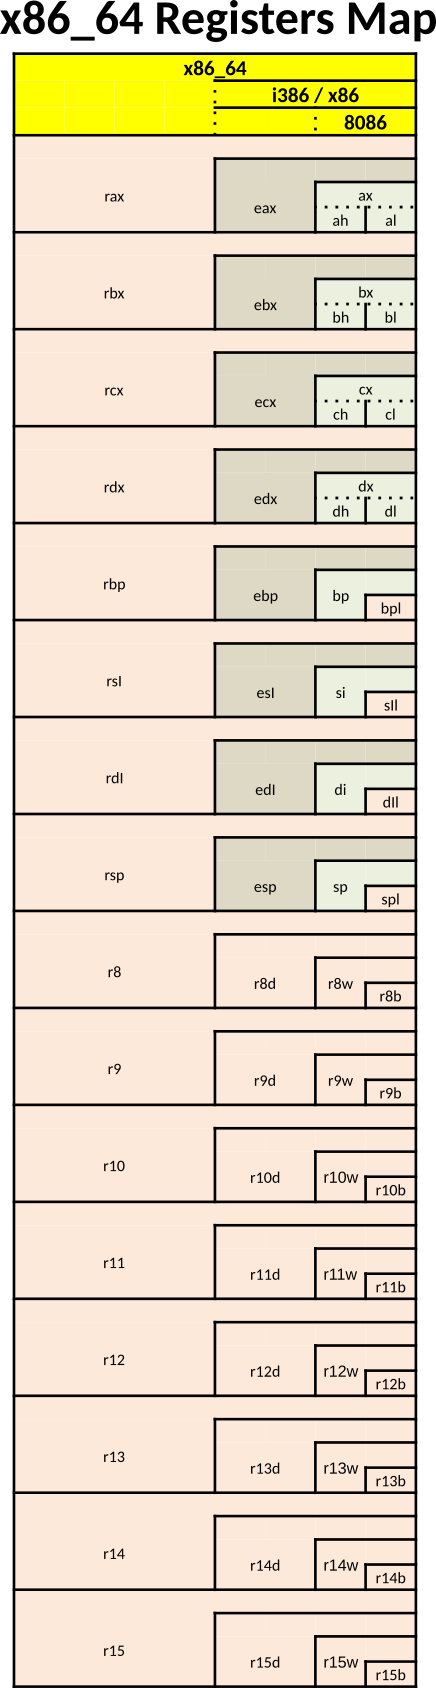
\includegraphics[height=9in]{../../02_Registers/images/X86_64-GP-registersBIG}
    

%\includegraphics[height=8in]{../../02}
\end{center}

%%%%%%%%%%%%%%%%%%%%%%%%%%%%%%%%%
\vspace{0.5in}
The following is probably a placeholder, and it won't show up on the exam version.\\
\begin{tabular}{|c|c|c|c|}
    \hline
   function & arguments & return value & notes\\    
    \hline
    puts & char *s & size\_t length & does not count null byte \\
    \hline
    strcpy & char *dest, char *src & char *dest & dest must be big enough \\
    \hline
    strncmp & char *s1, char *s2, size\_t n & int & 0 if equal, $<$0 if s1<s2, $>$0 if s1>s2 \\
    \hline
    strncpy & char *dest, char *src, size\_t n & char *dest & dest must be big enough \\
    \hline
    strcat & char *dest, char *src & char *dest & dest must be big enough \\
    \hline
    strncat & char *dest, char *src, size\_t n & char *dest & dest must be big enough \\
    \hline
    strcmp & char *s1, char *s2 & int & 0 if equal, $<$0 if s1<s2, $>$0 if s1>s2 \\
    \hline
\end{tabular}

\end{document} 